\section*{Appendix J: Experiments}
\label{app:experiments}

In this section, we empirically validate our theory using simulation results. In particular, we focus on three questions that mirror the main analytical claims:
\begin{enumerate}
    \item Does the coordination-first protocol produce substantially smaller regret than a naive decentralized baseline?
    \item Are collisions in fact concentrated in the short coordination stage, rather than persisting throughout learning?
    \item Does the local-peek step matter in practice, or could one simply rank cells by their center values?
\end{enumerate}

\paragraph{Experimental setup.}
We work in the partition-based collision model from Section~\ref{sec:setup}. In each run, the mean reward is a Lipschitz function on $[0,1]^d$ obtained from a small number of cone-shaped peaks. Observed rewards are Bernoulli with mean $\mu(x)$. Regret is measured against exactly the same benchmark used throughout the paper, namely the sum of the top-$N$ cell maxima from \eqref{eq:cont-regret}. We consider one-dimensional and two-dimensional instances, since these are the smallest settings in which both the geometric structure and the collision effects are easy to visualize.

The full experimental configuration is listed in Table~\ref{tab:exp-config}. Plots are averaged over $5$ random seeds and the shaded bands in the plots denote $95\%$ confidence intervals across seeds.

\paragraph{Methods compared.}
Since our paper proposes a new setting, we do not have a clear baseline to compare to. Thus, we consider the naive method where each player runs an independent single-agent Lipschitz bandit routine over the \emph{entire} domain and ignores the presence of the other players except through the collision-censored feedback as a natural starting point for comparison. Concretely, each player uses the same fixed-grid UCB primitive that our method uses in its final within-cell stage, but applies it globally rather than after coordination. This makes the comparison easy to read as the principal difference is not the local learning rule, but the presence or absence of an explicit coordination stage.

For this empirical study, we pool the successful Phase-I and Phase-II identification samples when forming the common target set. We do this to keep the experiments focused on the coordination-versus-learning decomposition that is central to the paper, rather than on incidental finite-sample disagreement between players during identification. The seating stage and the Phase-III local optimization stage are otherwise unchanged.

\begin{table}[t]
\centering
\small
\begin{tabular}{lccccccc}
\hline
Setting & $T$ & $N$ & Cells & $T_0$ & $T_1$ & Local grid & Seeds \\
\hline
1D regret & $10{,}000$ & $3$ & $8$ & $260$ & $700$ & $7$ & $5$ \\
2D regret & $10{,}000$ & $3$ & $4\times 4$ & $520$ & $1100$ & $5\times 5$ & $5$ \\
Pathology illustration & -- & $2$ & $6$ & -- & $9$ probes/cell & -- & deterministic \\
\hline
\end{tabular}
\caption{\textbf{Synthetic environments and algorithmic settings.} ``Local grid'' denotes the number of candidate points per cell used by the within-cell UCB routine in Phase III.}
\label{tab:exp-config}
\end{table}

\paragraph{Regret curves.}
Figure~\ref{fig:appendix-empirical-regret} reports cumulative regret in 1D and 2D. The qualitative picture is the same in both dimensions. The independent baseline repeatedly directs multiple players toward the same attractive cells and therefore accumulates regret at an essentially linear rate. By contrast, our protocol pays a short upfront price to identify distinct high-value cells and seat the players on them. Once that coordination cost has been paid, the learning problem largely decouples across players, and the subsequent regret growth is much slower.

\begin{figure}[t]
    \centering
    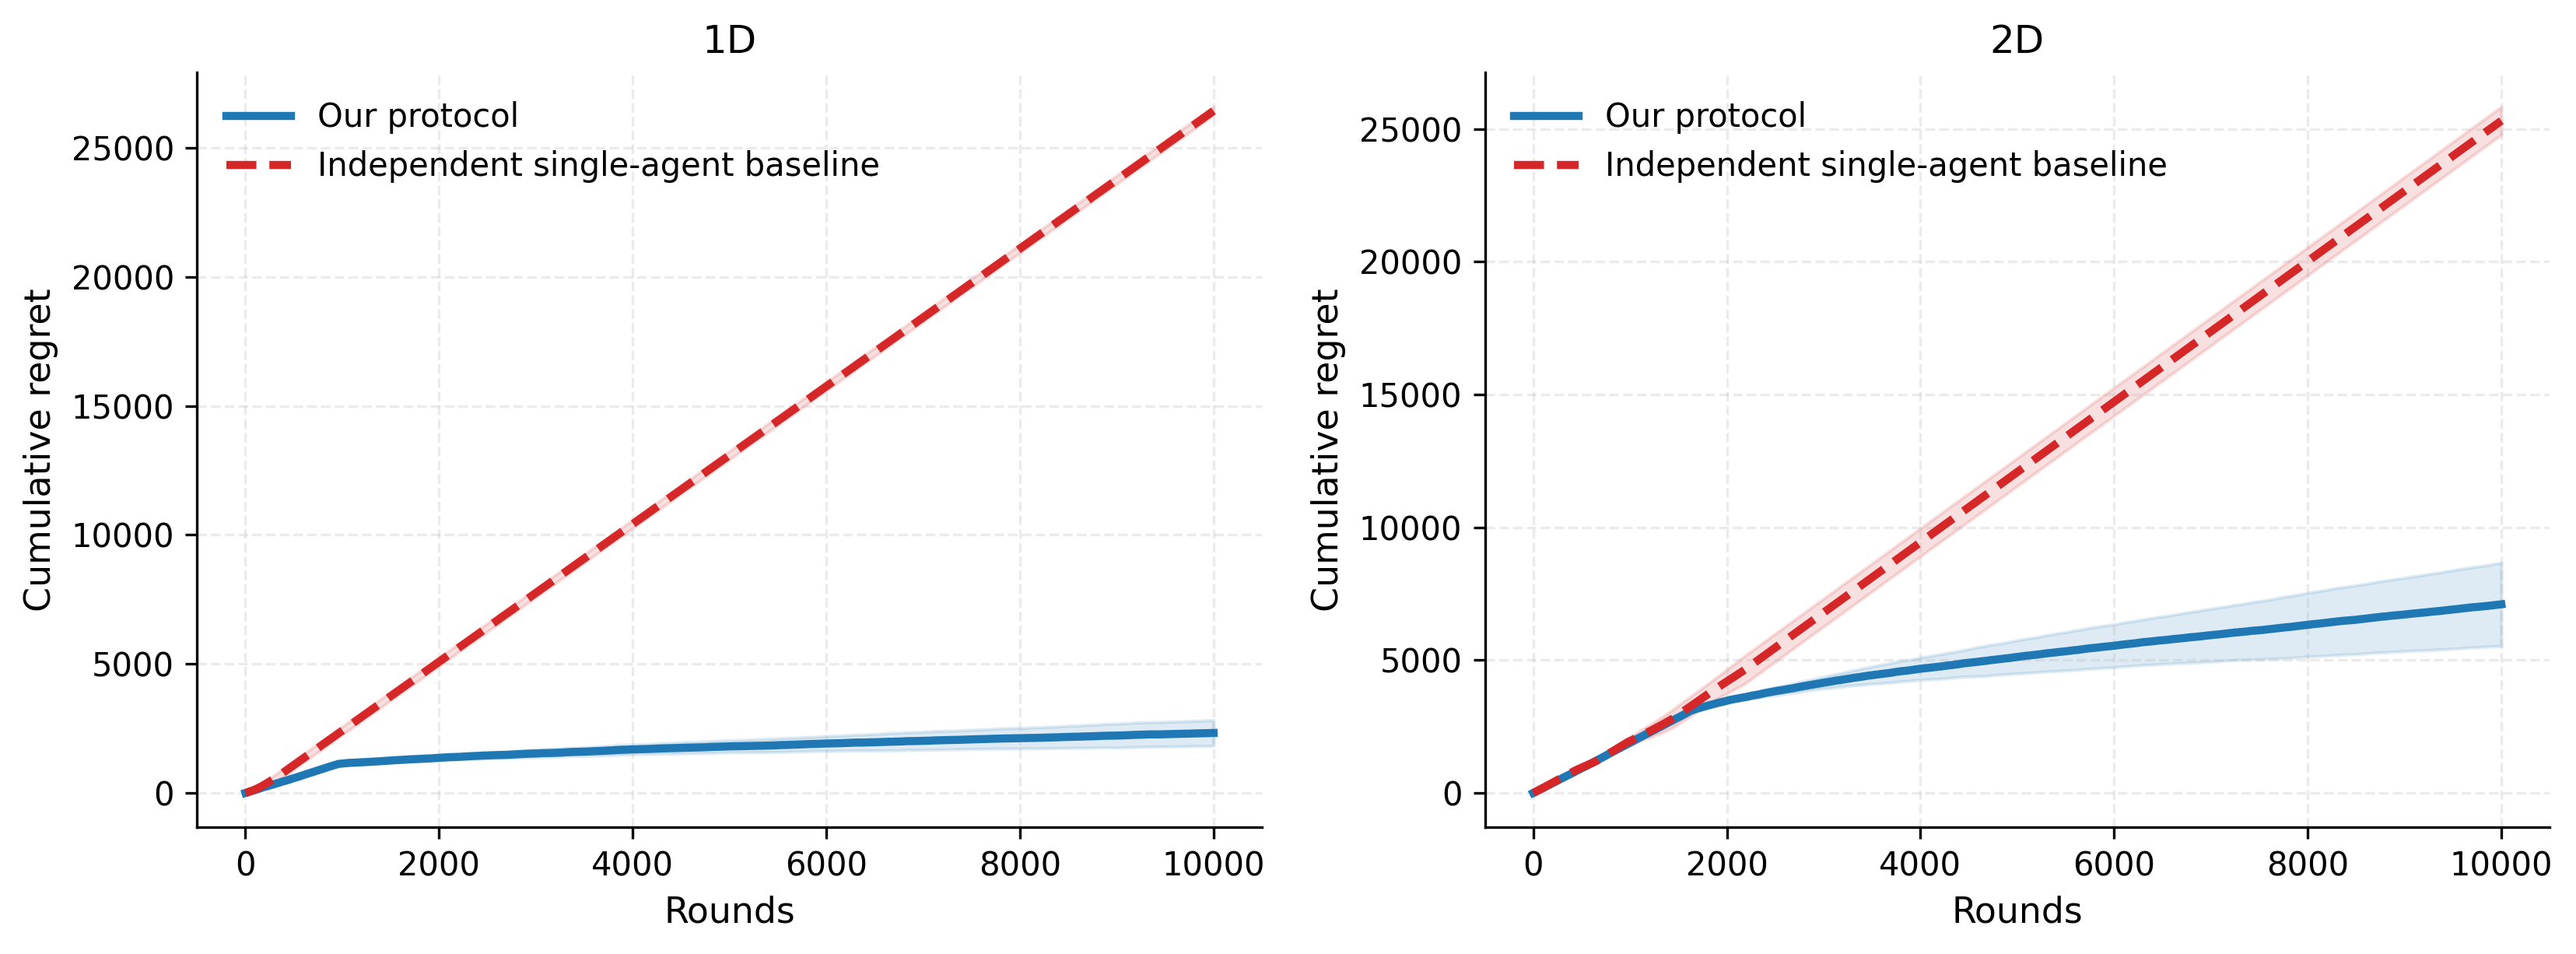
\includegraphics[width=0.99\linewidth]{empirical_regret_main.png}
    \caption{\textbf{Cumulative regret in simple synthetic instances.} We compare the proposed protocol against the independent single-agent baseline in 1D and 2D. Curves are averaged over $5$ random seeds and shaded bands denote $95\%$ confidence intervals. The baseline exhibits near-linear regret because players continue to collide on the same high-value cells, whereas the proposed protocol incurs a short coordination cost and then grows much more slowly.}
    \label{fig:appendix-empirical-regret}
\end{figure}

\begin{table}[t]
\centering
\small
\begin{tabular}{lccc}
\hline
Setting & Our protocol & Independent baseline & Mean seating rounds \\
\hline
1D at $T=10{,}000$ & $2326.2$ & $26432.4$ & $3.6$ \\
2D at $T=10{,}000$ & $7102.4$ & $25306.4$ & $2.2$ \\
\hline
\end{tabular}
\caption{\textbf{Final regret summary.} Values are mean cumulative regret at the final horizon in Figure~\ref{fig:appendix-empirical-regret}. The last column reports the average number of rounds spent in the seating stage by the proposed protocol.}
\label{tab:exp-summary}
\end{table}

\paragraph{Collision dynamics.}
The regret curves become easier to interpret once we inspect the collisions directly. Figure~\ref{fig:empirical-collisions} shows the smoothed fraction of colliding players over time, with vertical markers denoting the ends of Phase I and Phase II. The baseline keeps colliding throughout the run; every player is effectively trying to solve the same global problem, so there is no mechanism for persistent deconfliction. Our method behaves very differently. Collisions are concentrated in the short identification and seating stages, after which they nearly disappear once players occupy distinct cells. This is precisely the operational picture suggested by the theory where collisions are an upfront coordination cost.

\begin{figure}[t]
    \centering
    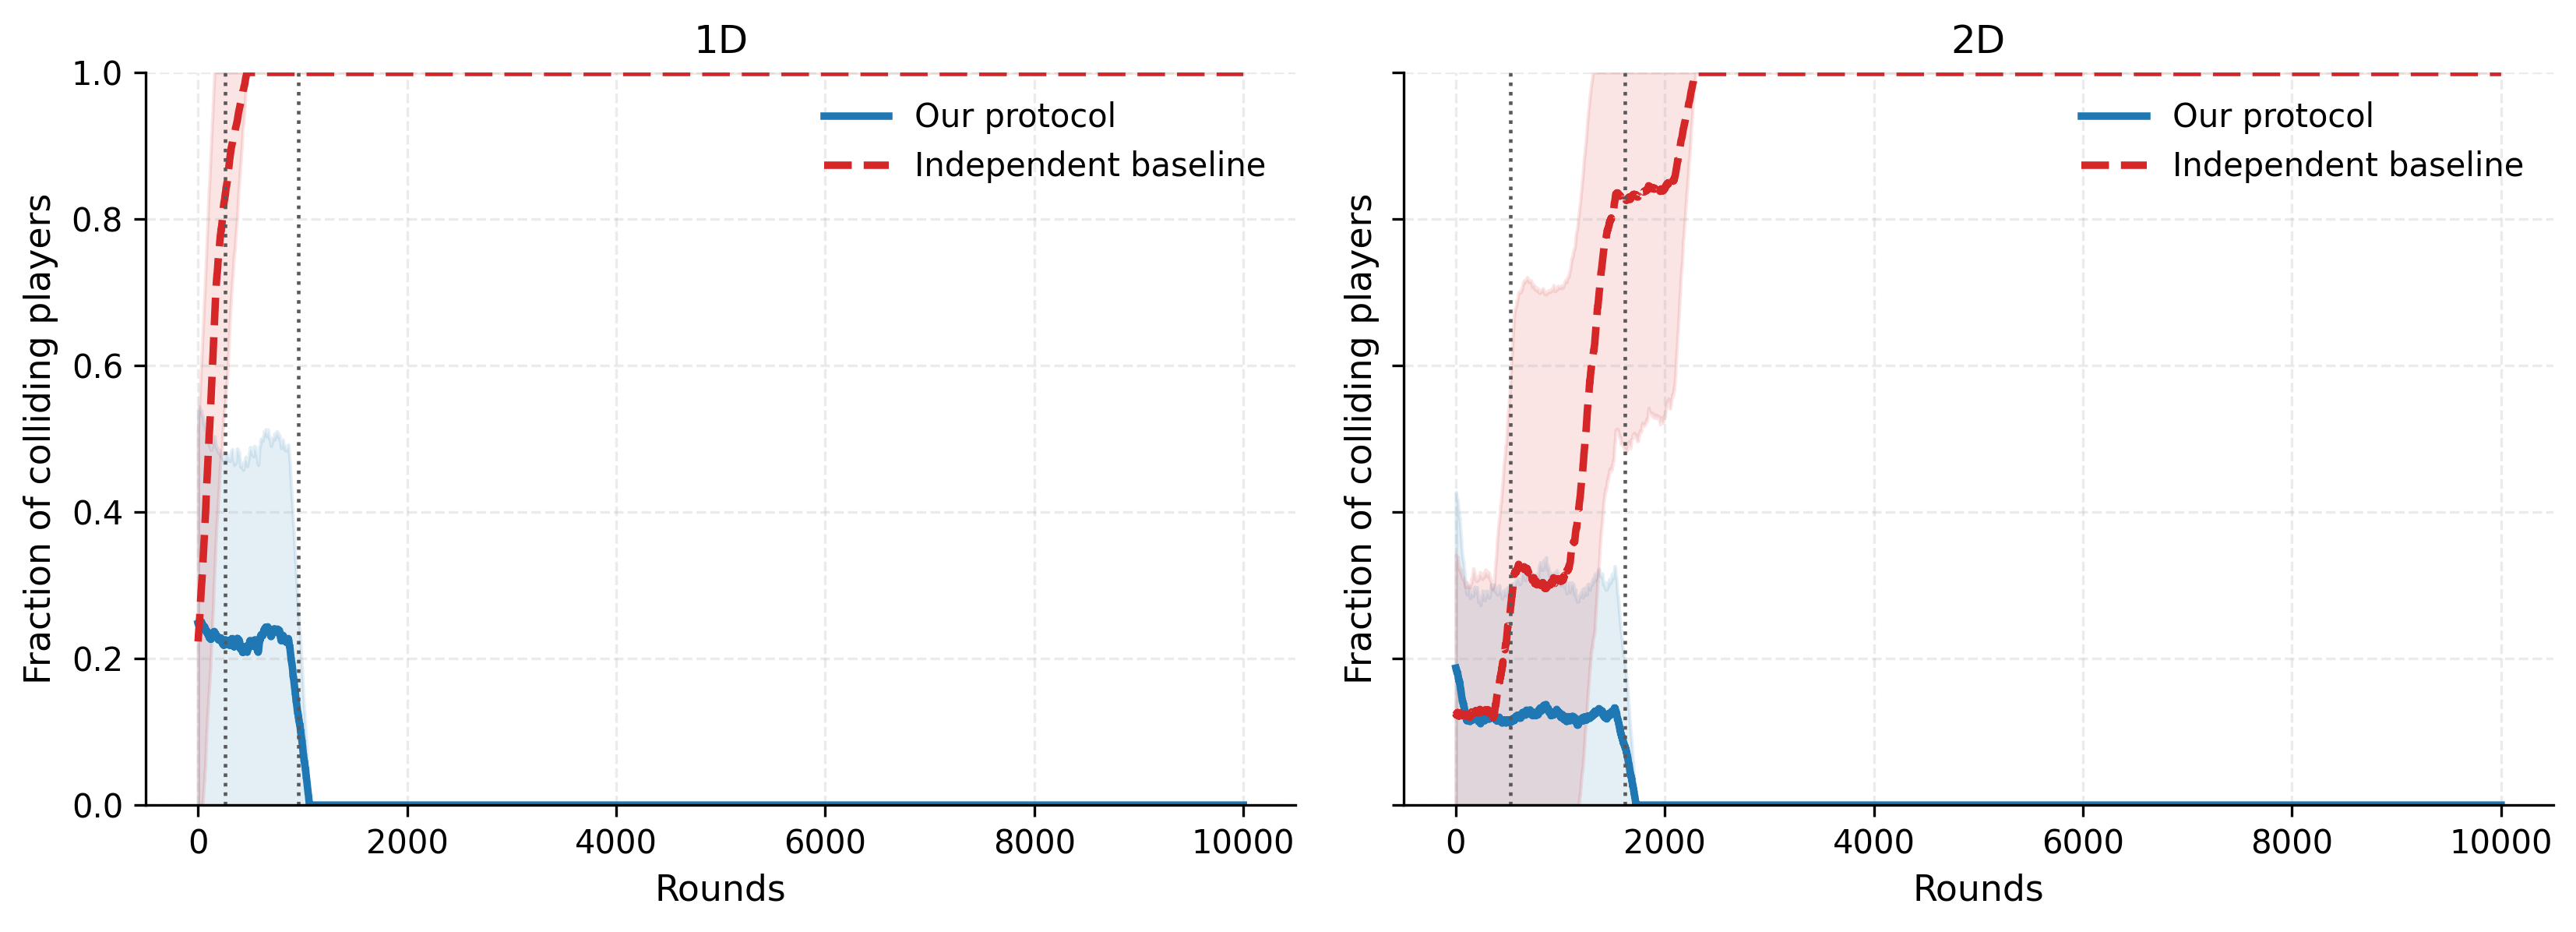
\includegraphics[width=0.99\linewidth]{empirical_collisions.png}
    \caption{\textbf{Collision traces in 1D and 2D.} Dotted vertical lines mark the ends of Phase I and Phase II. The proposed protocol localizes collisions to the short upfront coordination stage, while the independent baseline continues to collide almost all the time.}
    \label{fig:empirical-collisions}
\end{figure}


\paragraph{Why the local peek matters.}
Finally, Figure~\ref{fig:empirical-pathology} illustrates the specific geometric issue that motivates Phase II. The dominant peak lies very close to the boundary between cells $C_3$ and $C_4$. As a result, those two cells have the largest within-cell maxima, even though their center values are not the largest. In this instance, center-based ranking prefers $C_5$ and $C_6$ because their centers happen to lie in moderately strong regions, while the true top-$N$ cells are actually $C_3$ and $C_4$. The local-peek scores correct this mis-ranking by probing within each cell and therefore recover the correct pair.

\begin{figure}[t]
    \centering
    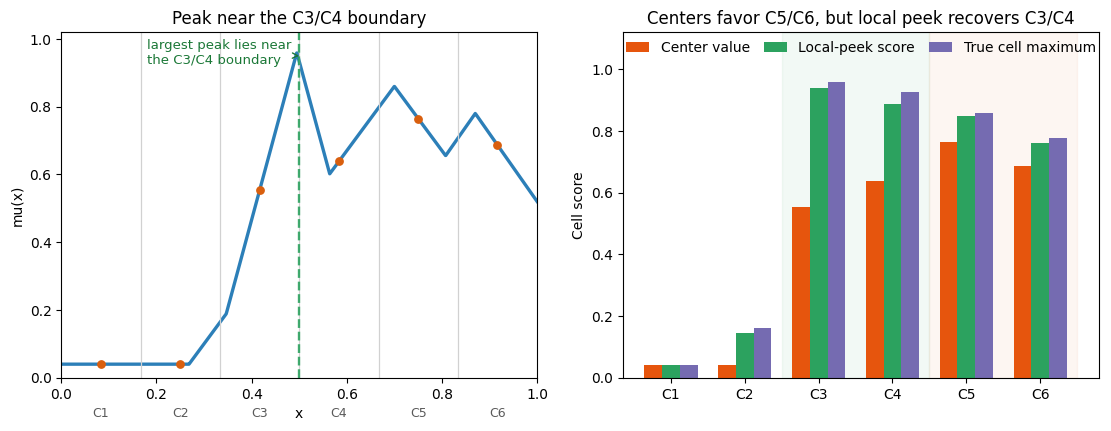
\includegraphics[width=0.99\linewidth]{empirical_pathology.png}
    \caption{\textbf{Boundary-peak pathology.} Left: a one-dimensional reward function in which the largest peak lies near the boundary between $C_3$ and $C_4$; orange markers denote the cell centers. Right: orange bars are center values, green bars are local-peek scores, and purple bars are true cell maxima. The center values are largest for $C_5$ and $C_6$, so a center-based ranking would choose those cells. In contrast, the true cell maxima are largest for $C_3$ and $C_4$, and the local-peek scores recover exactly that ordering. This is the geometric failure mode that motivates Phase II.}
    \label{fig:empirical-pathology}
\end{figure}

Taken together, these experiments support the main qualitative message of the paper. The primary difficulty in this setting is the need to coordinate players onto different high-value regions without communication. Once that coordination is handled, the remaining learning problem behaves much more like a collection of ordinary single-player Lipschitz bandits.

All figures in this appendix can be regenerated from the repository at: https://github.com/amitrege/aistats\_multiagent\_code 
